	\section{Цель работы:}
		Изучить рекомендации MSF по построению диаграмм вариантов использования системы. Подготовить модель вариантов использования.
	\section{Порядок выполенения работы:}
		\subsection{Описание системы}
			В данной работе рассматривается задача реализации системы моделирования Динамических вычислительных сетей.
			
			\textit{Динамические вычислительные сети} (далее ДВС) -- обобщение формализма сетей Петри, характеризующееся:
			\begin{itemize}
				\item изменением структуры сети во времени,
				\item осуществлением переходов в реальном времени,
				\item «вычислительной» нагрузкой переходов в сети.
			\end{itemize}

		\subsection{Определение главных и второстепенных актеров, и определение цели главных актеров по отношению к системе}
			Единственным действующим лицом в данной системе может быть ДВС-проектировщик. Его задачи:
			\begin{enumerate}
				\item cоставление модели ДВС.
				\item проверка модели на корректность.
				\item моделирование процесса в ДВС. 
			\end{enumerate}
			
			Цель ДВС-проектировщика -- создать такую ДВС модель, которая корректно моделировала бы некоторый параллельный процесс.
		\subsection{Основные варианты использования, которые специфицируют функциональные требования к системе}
			При анализе задачи выявлены следующие варианты использования:
			\begin{itemize}
				\item возможность создания модели ДВС,
				\item возможность редактирования этой модели,
				\item возможность сохранения модели,
				\item возможность загрузки модели,
				\item проверка корректности составленной модели,
				\item моделирование процесса в ДВС,
				\item просмотр истории изменения маркировки сети.
			\end{itemize}
			\vspace{\baselineskip}
			Отсортируем их в порядке убывания степени риска:
			\begin{enumerate}
				\item моделирование процесса в ДВС,
				\item проверка корректности составленной модели ДВС,
				\item возможность создания модели ДВС,
				\item возможность редактирования этой модели,
				\item просмотр истории изменения маркировки сети,
				\item возможность сохранения модели,
				\item возможность загрузки модели.
			\end{enumerate}
			\clearpage
			
		\subsection{Cценарий реализации выбранного варианта использования}
			Выберем вариант использования № 1. моделирование процесса в ДВС.
			
			\begin{center}
				\begin{tabular}[t]{|p{0.4\linewidth}|p{0.4\linewidth}|}
					\hline
					\textbf{Действия актера} 
						& \textbf{Отклик системы} \\ 
					\hline
					Открыть некоторую сеть для просмотра &  \\ 
					\hline
					Запустить моделирование, если сеть построена корректно.\vskip20pt
					\textbf{Исключение 1:} сеть построена некорретно.
						& 1. Проверить, корректна ли данная сеть Петри\newline
						2. Анимация процесса в ДВС.\\
					\hline
				\end{tabular}
			\end{center}
			
			\vskip20pt
			\begin{center}
				\begin{tabular}[t]{|p{0.4\linewidth}|p{0.4\linewidth}|}
					\hline
					\multicolumn{2}{|c|}{\textbf{Исключение 1:} сеть построена некорретно.}\\
					\hline
					\textbf{Действия актера} 
						& \textbf{Отклик системы} \\ 
					\hline
						& Отобразить сообщение о некорректно построенной сети. \\ 
					\hline
				\end{tabular}
			\end{center}
			
		\begin{landscape}
		\subsection{Диаграмма ВИС}
			\begin{figure}[h!]
				\center{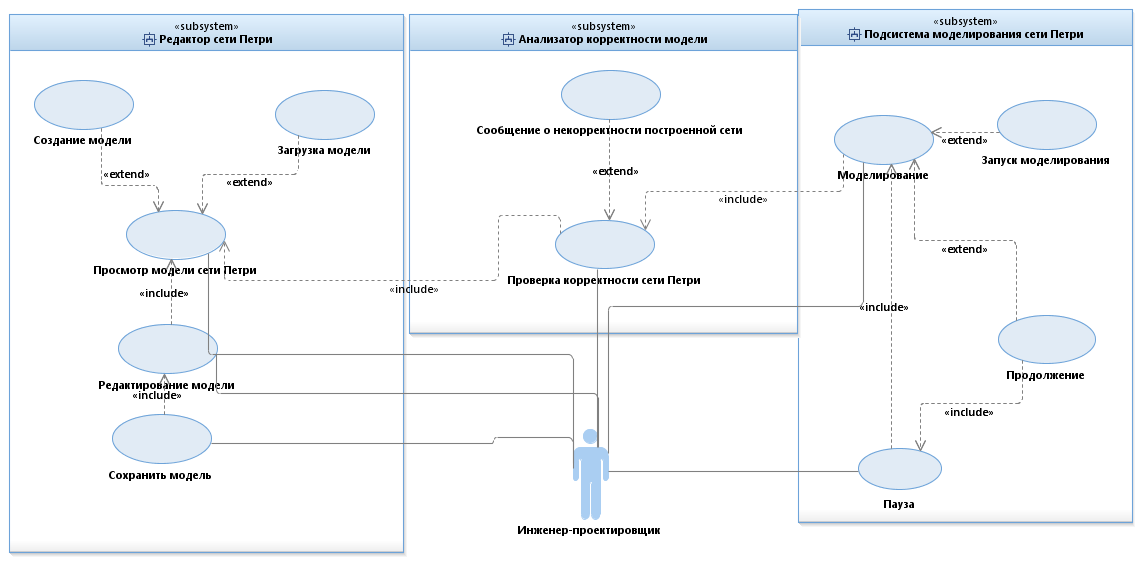
\includegraphics[width=0.7\paperheight]{UML}}
				\caption{Диаграмма вариантов использования}
				\label{uml}
			\end{figure}
		\end{landscape}
	